

\chapter{Key Distribution and Key Exchange}
	
\section{Private Key Cryptography}
	\begin{center}
		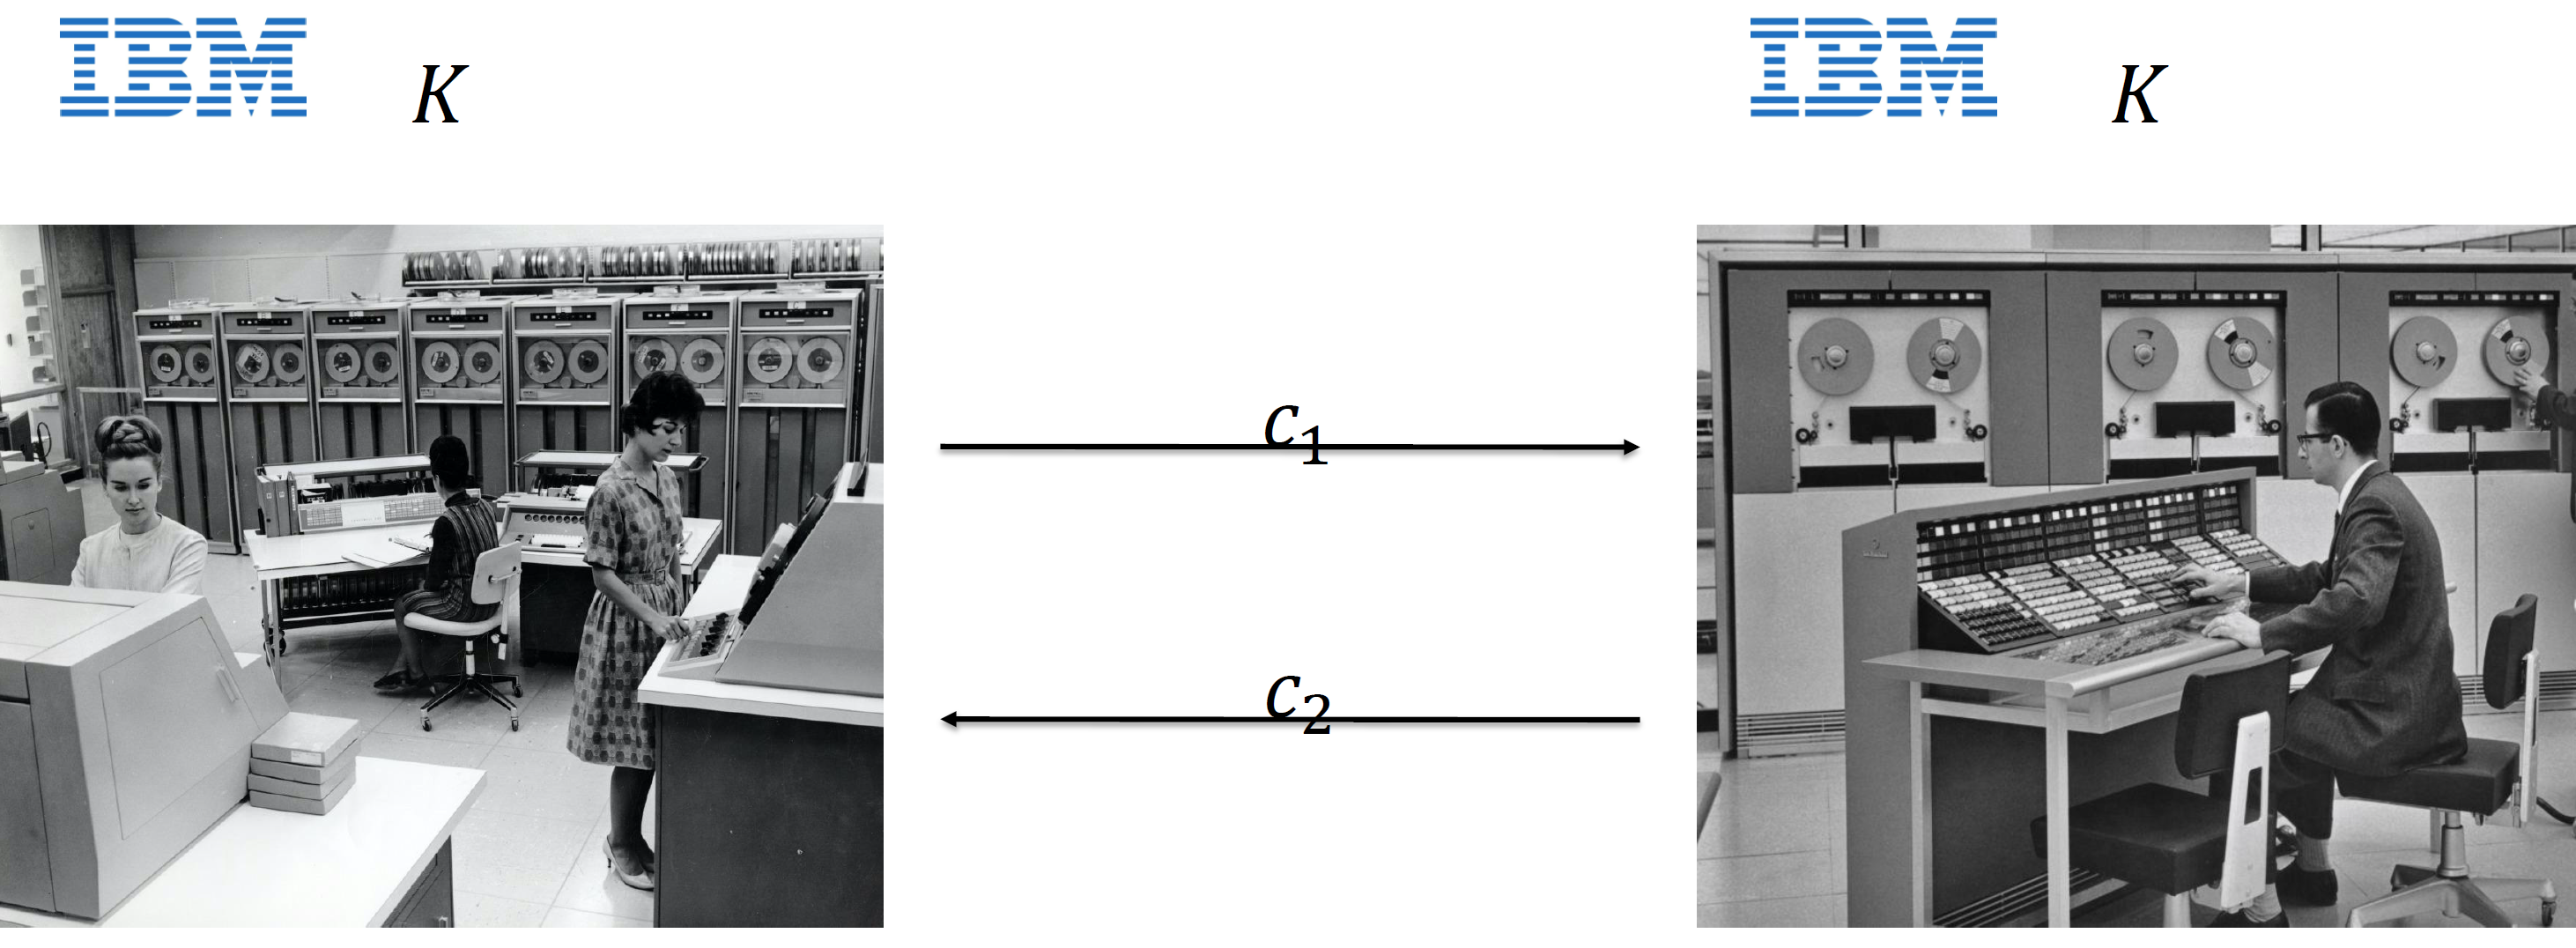
\includegraphics[width=140mm]{Graphics/Key Distribution and Key Exchange/kdke1.png}
	\end{center}

\section{A modest Proposal: Key Distribution Centers}
	\begin{itemize}
		\item Central Entity the manages and distributes keys
		\item Each user has a joint key with key distribution center (KDC)
		\item All keys can be computed pseudorandomly, KDC then only needs to store PRF key
		\item A establishes secure channel to B by requesting session key from KDC
		\item Major problem: KDC is single point of failure
		\item Compromising KDC compromises all other channels in the network
	\end{itemize}
	\begin{center}
		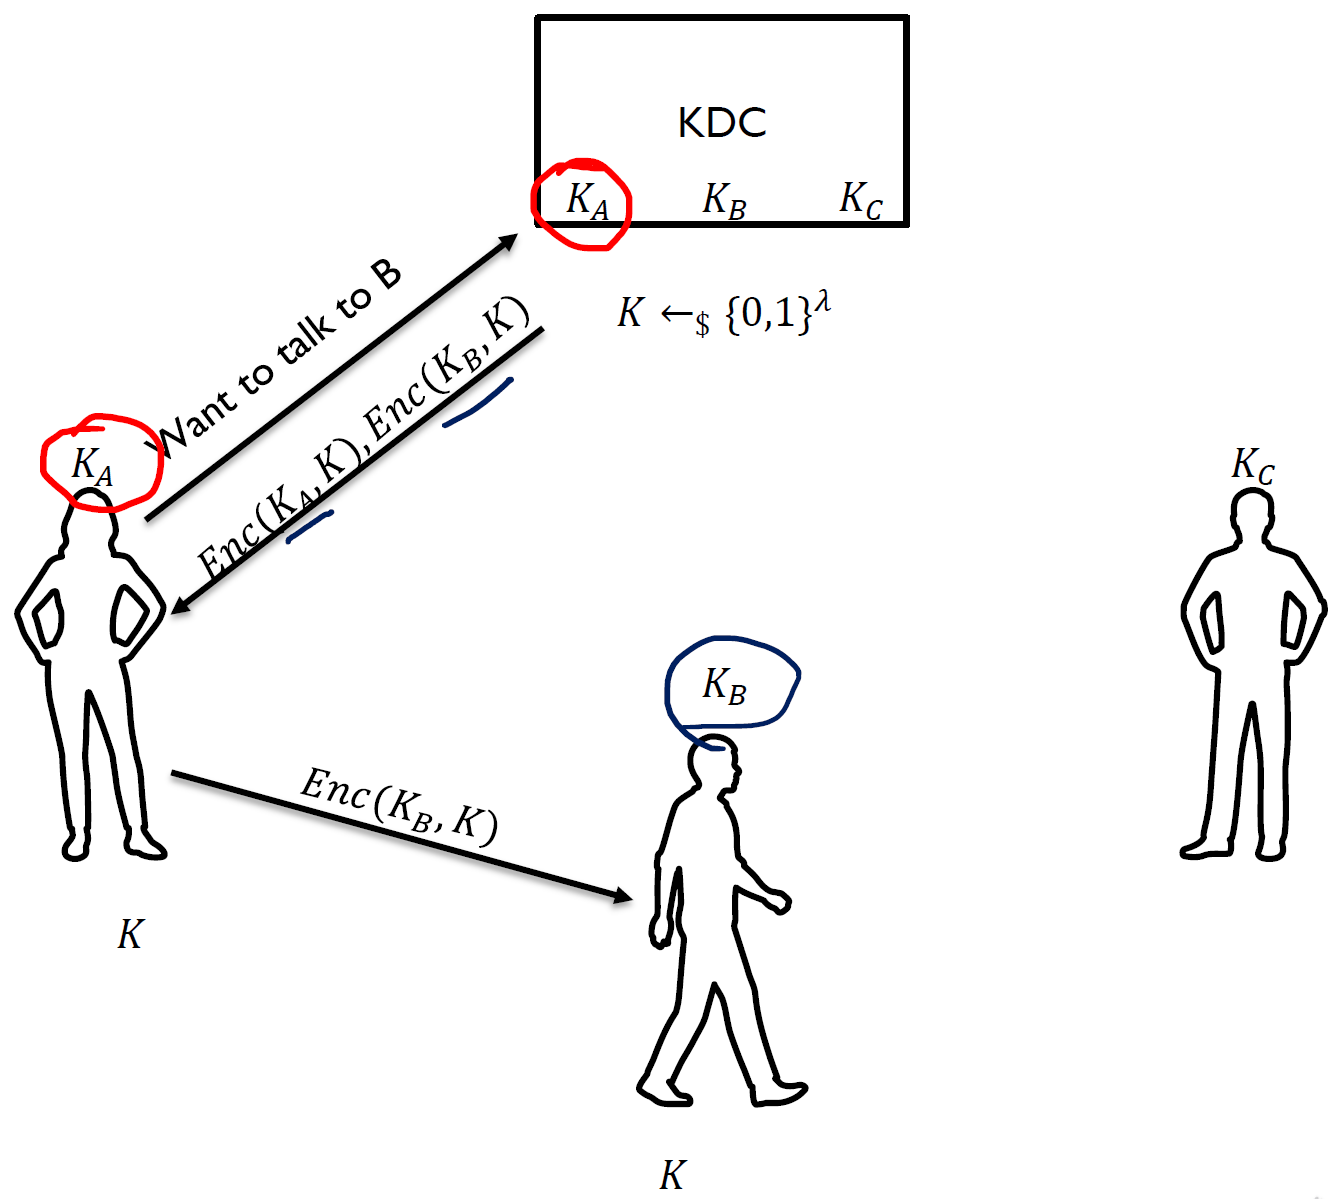
\includegraphics[width=100mm]{Graphics/Key Distribution and Key Exchange/kdke2.png}
	\end{center}

\section{New Directions in Cryptography}
	\begin{itemize}
		\item KDCs don’t solve key distribution problemin open systems
		\item Observation of Diffie and Hellman: Many physical processes are asymmetric
		\item E.g. Padlock, shattering glass
		\item "Easy" in one direction, "hard" in the other
		\item Idea: exploit a computational phenomenon with this property to remotely establish a key
	\end{itemize}
	\begin{center}
		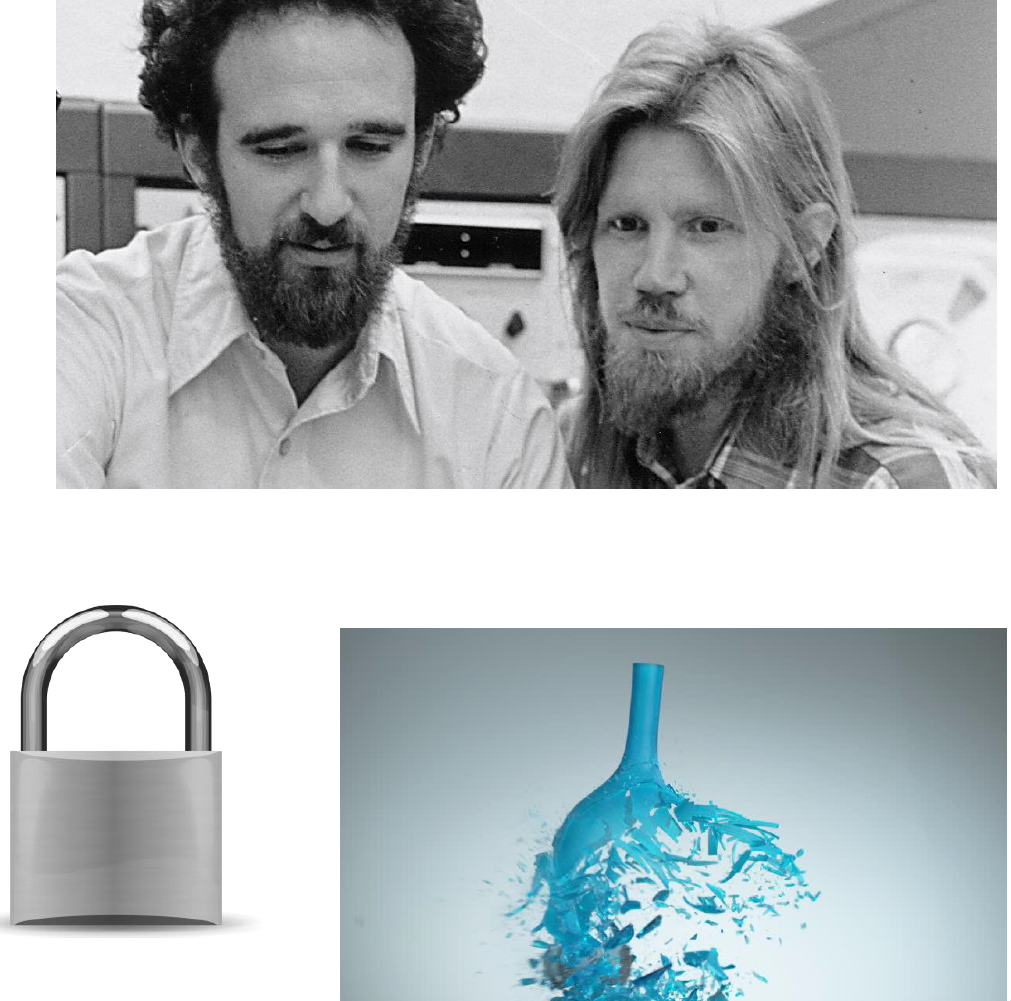
\includegraphics[width=100mm]{Graphics/Key Distribution and Key Exchange/kdke3.png}
	\end{center}

\section{Diffie-Hellman Key Exchange}
	\begin{itemize}
		\item Recall: Mechanism to generate cryptographic group $\mathcal{G}$ of order $p$ with generator $g$
		\item $(\mathcal{G},\cdot)$
	\end{itemize}
	\begin{center}
		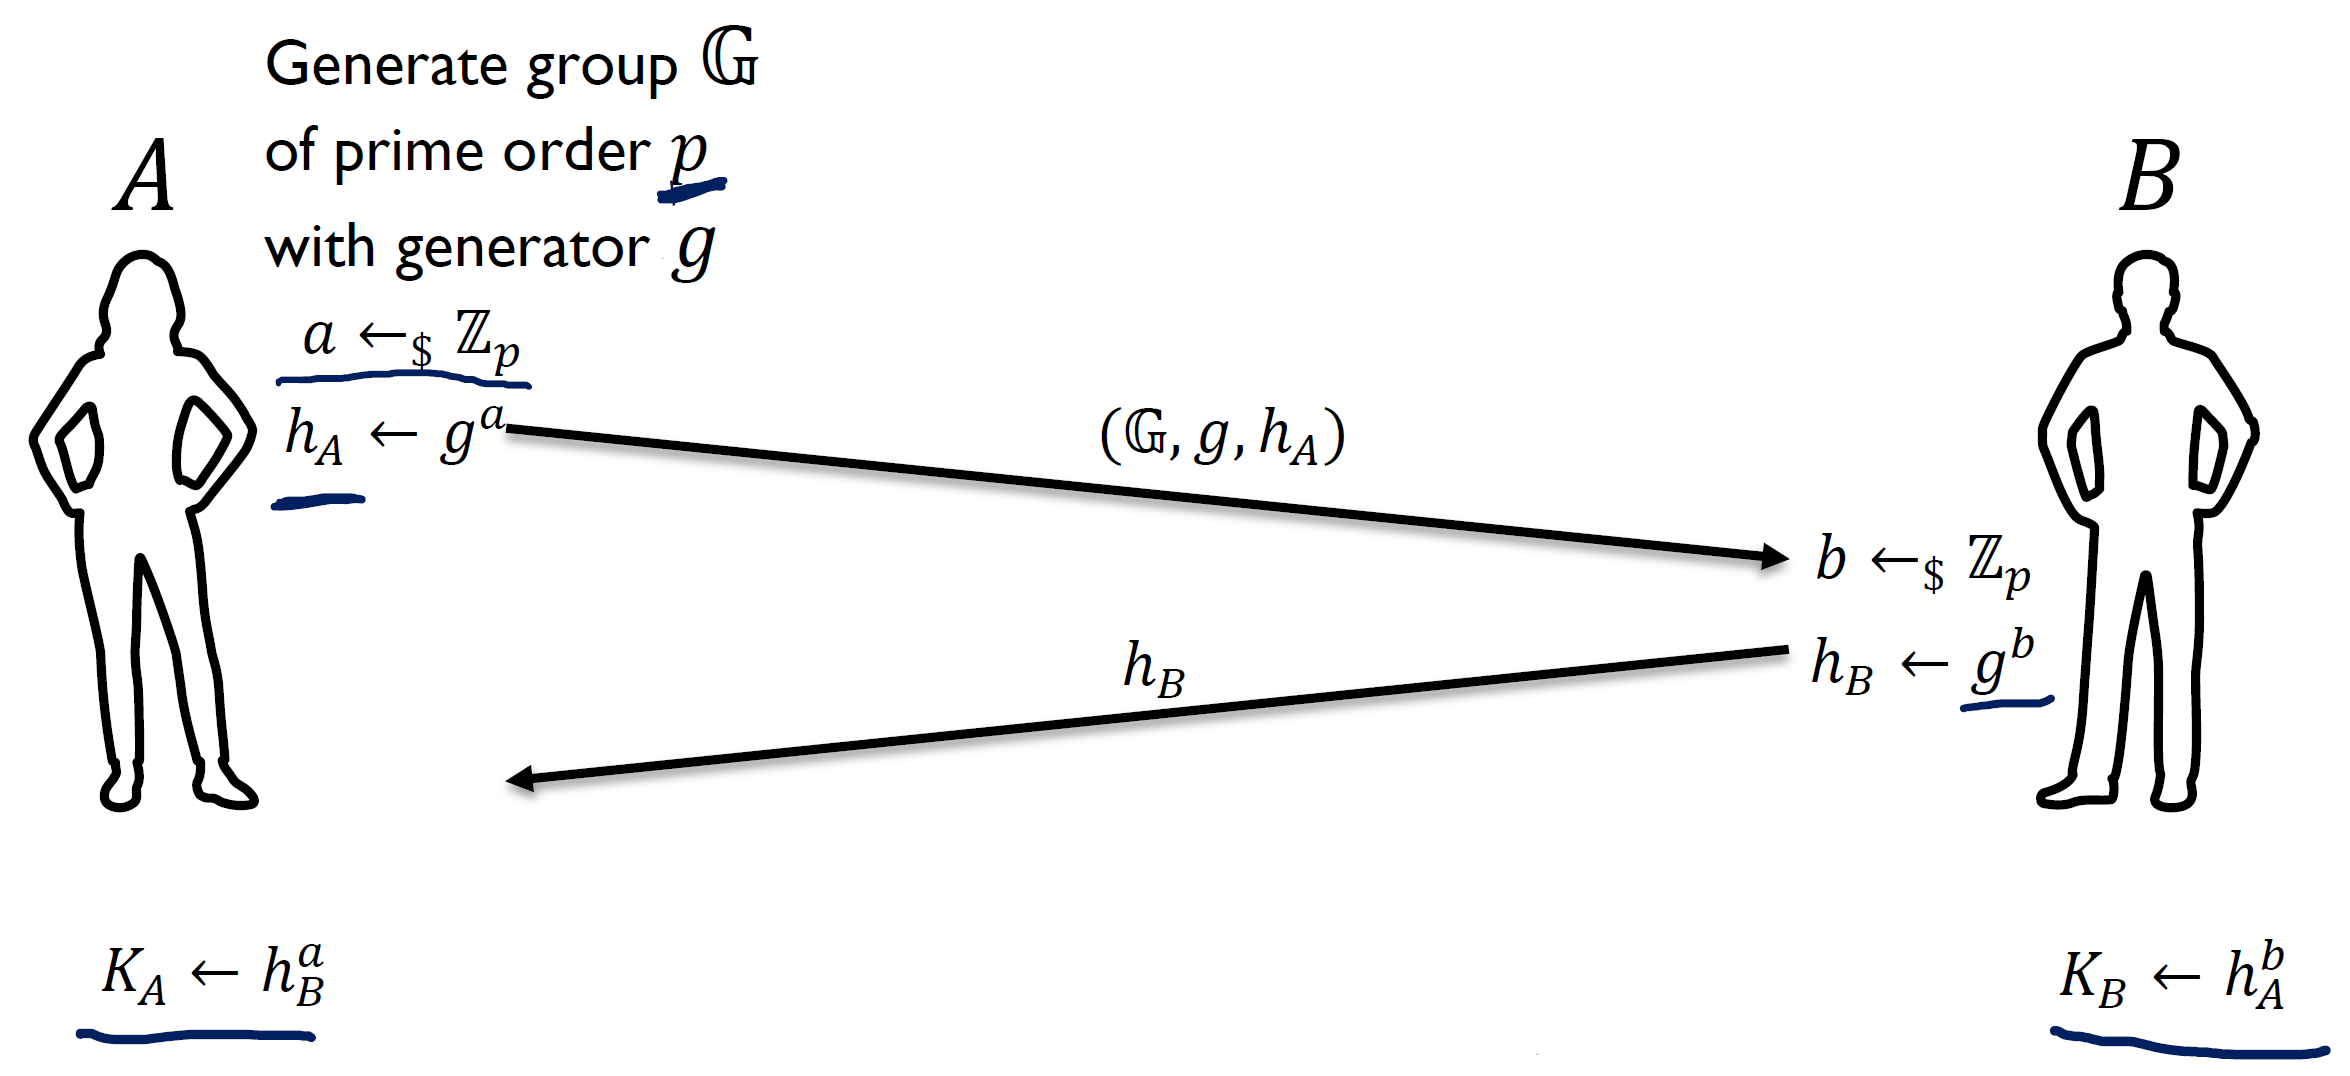
\includegraphics[width=100mm]{Graphics/Key Distribution and Key Exchange/kdke4.png}
	\end{center}
	$$K_A = h^a_B = (g^b)^a = g^{ab} = (g^a)^b = h^b_A = K_B$$

\section{Formal Definitions for Key-Exchange Protocols}
	\begin{itemize}
		\item Key exchange protocol $\Pi$ consists of algorithms/instructions for Alice and Bob which output private state and output-message
		\item Let $T$ denote the public transcript of the protocol
		\item Write $(T,K) \leftarrow \Pi(1^{\lambda})$ to denote a run of the protocol $\Pi$ (with uniformly random coins) which results in a transcript $T$ and a key $K$
		\item E.g. for Diffie-Hellman key-exchange: $\Pi = (Alice_1, Bob, Alice_2)$
		\begin{itemize}
			\item $Alice_1(1^{\lambda}) \rightarrow ((\mathbb{G},a),(\mathbb{G},g,h_a))$ with $h_A = g^a$
			\item $Bob(\mathbb{G},g,h_A) \rightarrow (K_B,K_B)$
			\item $Alice_2 ((\mathbb{G},a),h_B) \rightarrow K_A$
			\item $T = (\mathbb{G},g,h_A,h_B)$
		\end{itemize}
		\item \textbf{Correctness:} $Pr[K_A = K_B] = 1$
	\end{itemize}

\section{Security Definition for Key Exchange}
	\begin{itemize}
		\item Let $\Pi$ be a key-exchange protocol.
		\item $(T,K) \leftarrow \Pi(1^{\lambda})$
		\item Let $\hat{K} \leftarrow_{\$} \{0,1\}^{\lambda}$ be chosen uniformly random
		\item We say that $\Pi$ is \textit{secure against eavesdropping}, if ith holds for every PPT distinguisher $\mathcal{D}$ that
		$$|Pr[\mathcal{D}(T,K) = 1] - Pr[\mathcal{D}(T,\hat{K} = 1]| \leq negl(\lambda)$$
		\item Probability taken over the choice of $T,K$ and $\hat{K}$
	\end{itemize}
	\begin{center}
		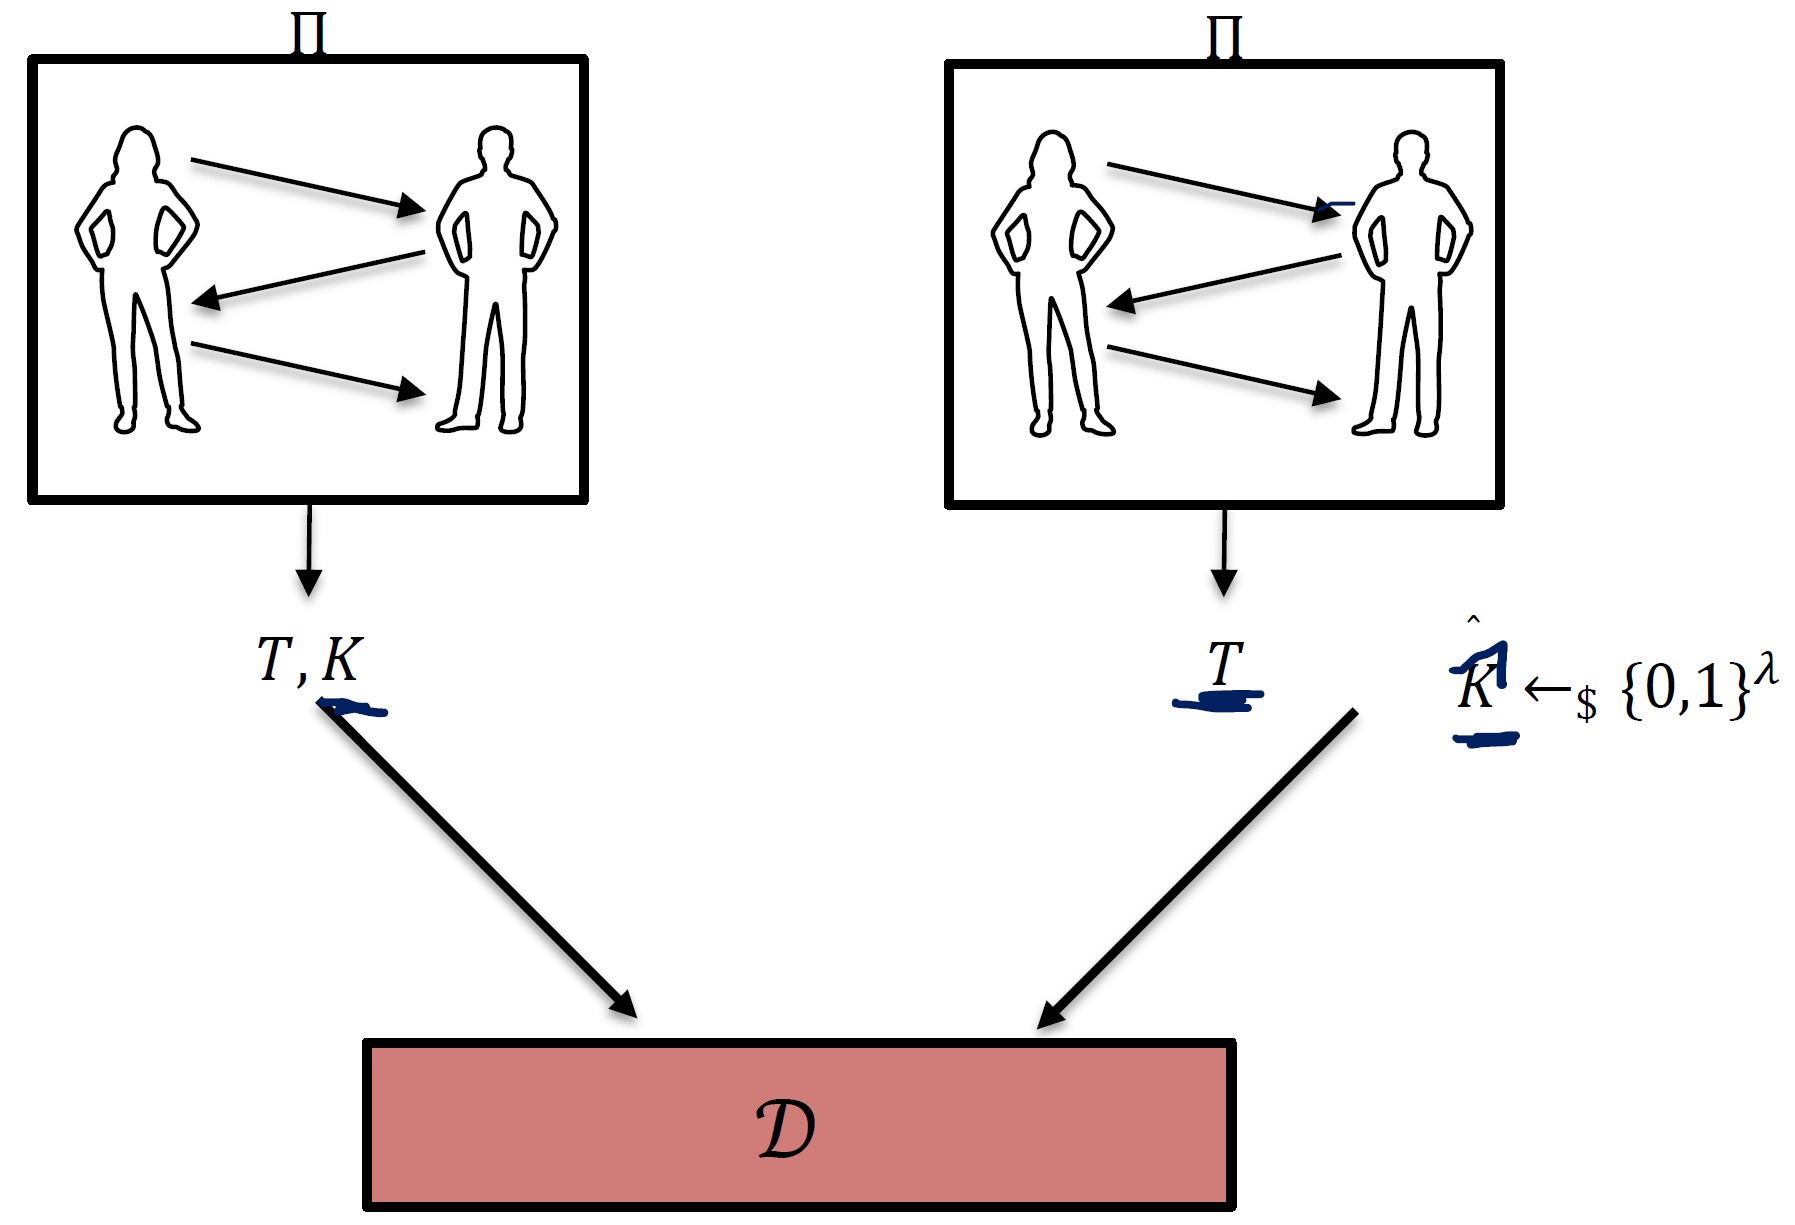
\includegraphics[width=120mm]{Graphics/Key Distribution and Key Exchange/kdke5.png}
	\end{center}

\section{The Decisional Diffie-Hellman (DDH) Assumption}
	\begin{itemize}
		\item DDH Assumption: The Difiie-Hellman Key-Exchange protocol is secure against eavesdropping
		\item $a,b,r \leftarrow_{\$} \mathbb{Z}_p$
	\end{itemize}
	$$(\mathbb{G},g,g^a,g^b,g^{ab}) \approx (\mathbb{G},g,g^a,g^b,g^r)$$
	We assume the group $\mathbb{G}$ is fixed, so
	$$(g,g^a,g^b,g^{ab}) \approx (g,g^a,g^b,g^r)$$

\section{Summary}
	\begin{itemize}
		\item Private key encryption is useful in closed systems with pre shared keys
		\item In open systems we need a key distribution mechanism
		\item KDCs offer a partial solution
		\item Key exchange protocols offer a scalable solution
	\end{itemize}























